% !TEX root = SystemTemplate.tex

\chapter{Overview and concept of operations}


\section{Scope}
This document will provide an overview of the develolpment of the testing software.


\section{Purpose}
This product will compile and test c++ programs against predefined test cases.


\subsection{Major System Component \#1}
Location of existing, applicable test cases for the program needing to be tested.

\subsection{Major System Component \#2}
Run and test of a single program against located test cases

\subsection{Major System Component \#3}
Record and summary of test results

\section{Systems Goals}
The goal of this system is to provide an automated testing application, designed specifically
for professors testing submitted student programs. A user will be able to use the application
to test a desired program against all applicable test cases the application can find in the directory tree 
related to that program.  A time-stamped record will be created to summarize the output of each test and to provide a
general summary of the results. 

\section{System Overview and Diagram}
The major system components listed above will, upon completion, combine to create this testing application. 
Upon running the application and providing it with the name of the desired target program, the application
will complete the desired system goals via its major components.
\\ First, existing, applicable test cases will be found for the program needing to be tested. 
\\ Second, the program will be run against each test case input, and the resulting output will be 
compared to each desired test case output.
\\  Last, the program will create a time-stamped record for each program tested, providing a reference of 
the output results and a numerical summary of the overall success rate.  
\\ See Figure~\ref{systemdiagram}.
\begin{figure}[H]
\begin{center}
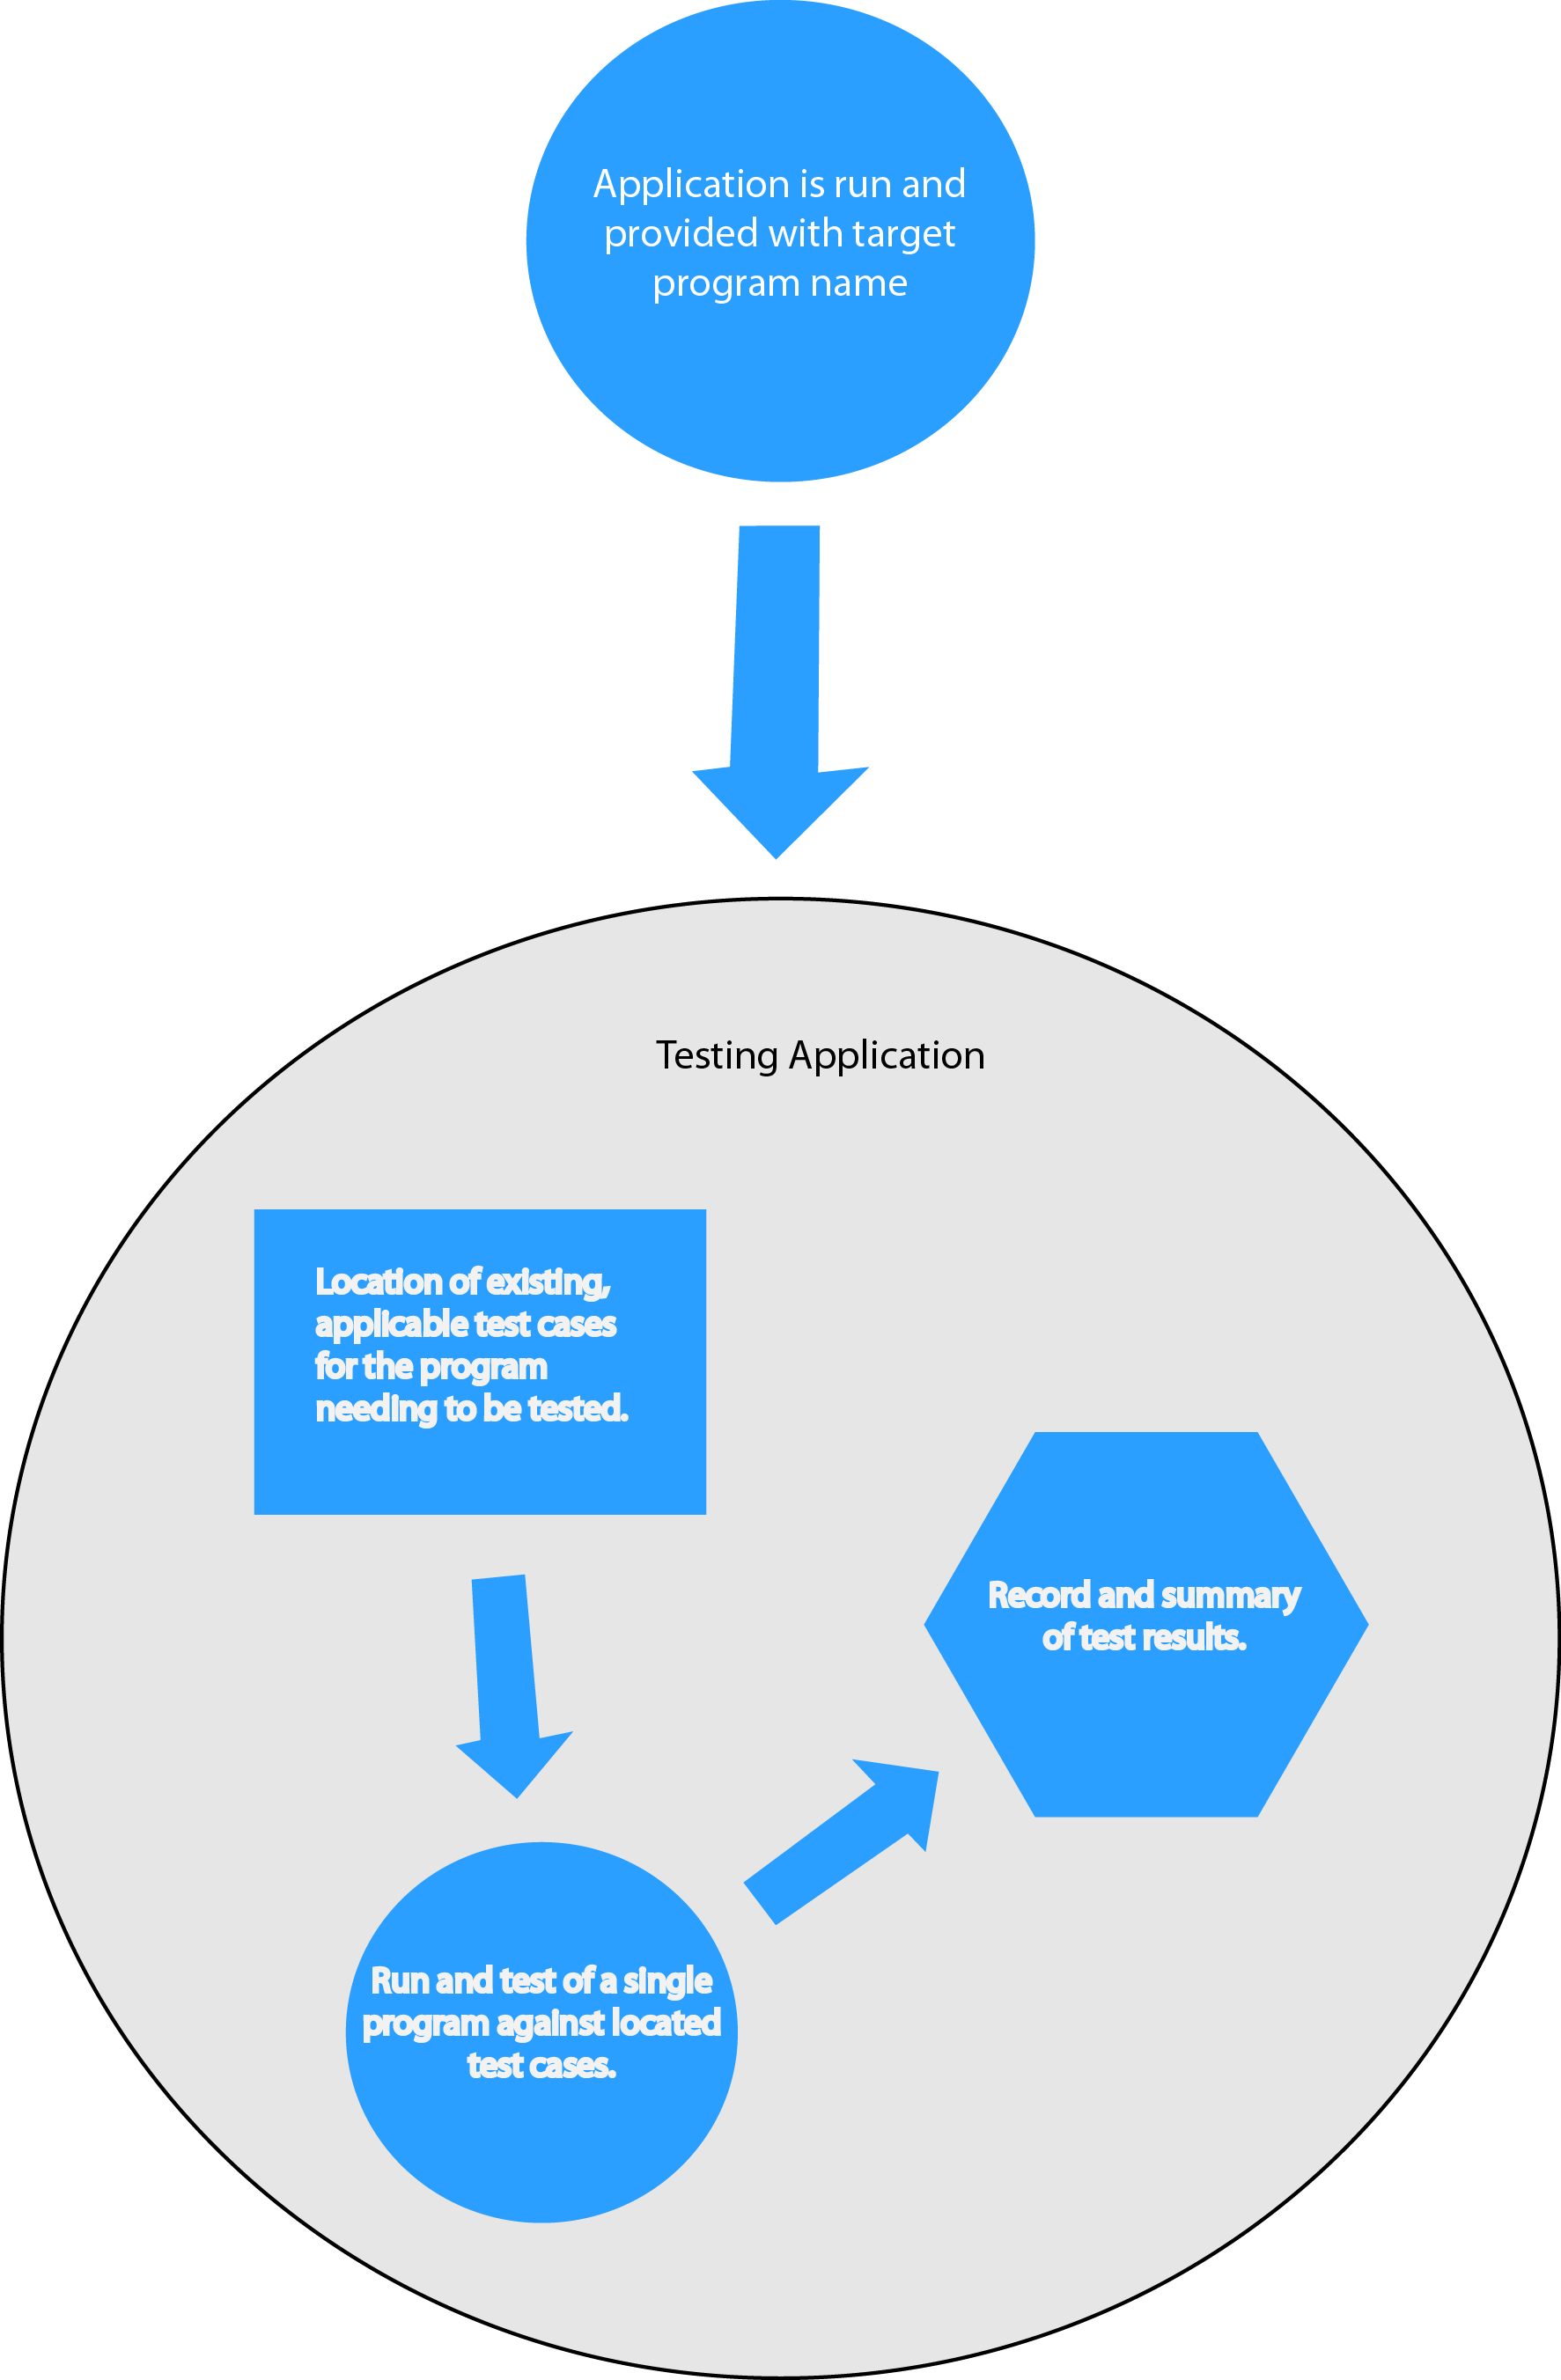
\includegraphics[width=0.9\textwidth]{./diagram}
\end{center}
\caption{The Testing System Diagram \label{systemdiagram}}
\end{figure}



\section{Technologies Overview}
The development team used the Agile Software Development Method, via the Scrum framework, to develop
this system.  This incremental development menthod was the required development method for this project.
Since the system was expected to created for a Linux platform, it was written and tested on a Linux Platform 
using Qt Creator.  The latter was picked as the Integrated Development Environment of the system, based on
the requirement that it be written in the programing language C++.
See Table~\ref{DevelopmentTable}.  
\begin{table}[tbh]
\begin{center}
\begin{tabular}{|r|l|}
  \hline
  Software Development Method & Agile Software Development Method \\
  Planning and Organization & Trello Project Management Application \\
  \hline \hline
  Platform & Linux \\
  Language & C++ \\  
  IDE & Qt Creator \\
  Version Control & Git and Bitbucket
  \\ \cline{2-2}
  
  \hline
\end{tabular}
\caption{The Development Methods and Technologies Table \label{DevelopmentTable}}
\end{center}
\end{table}

